%=============================================================================
%  Kalman Multi-Step Forecaster — Mathematical Notes & Documentation
%  Study Notes + Technical Reference | Dark Wing Project
%=============================================================================
\documentclass[10pt,a4paper,twocolumn]{article}

\usepackage[a4paper,top=1.8cm,bottom=1.8cm,left=1.5cm,right=1.5cm,columnsep=0.7cm]{geometry}
\usepackage{amsmath,amssymb,amsthm,mathtools}
\usepackage[T1]{fontenc}\usepackage{lmodern}\usepackage{microtype}
\usepackage{parskip}\setlength{\parskip}{2pt}
\usepackage{xcolor}
\definecolor{codebg}{RGB}{245,247,250}\definecolor{codeframe}{RGB}{180,195,220}
\definecolor{keyword}{RGB}{0,80,180}\definecolor{comment}{RGB}{80,115,80}
\definecolor{string}{RGB}{160,40,20}\definecolor{mathbluebg}{RGB}{230,240,255}
\definecolor{mathblue}{RGB}{10,60,160}\definecolor{accent}{RGB}{25,95,195}
\definecolor{greenbg}{RGB}{230,250,232}\definecolor{greenframe}{RGB}{50,155,70}
\definecolor{yellowbg}{RGB}{255,252,230}\definecolor{yellowframe}{RGB}{180,150,0}
\definecolor{notebg}{RGB}{248,245,255}\definecolor{noteframe}{RGB}{120,80,180}
\usepackage{listings}
\lstdefinestyle{pythonplain}{language=Python,backgroundcolor=\color{codebg},
  frame=single,rulecolor=\color{codeframe},basicstyle=\ttfamily\fontsize{6.5}{8}\selectfont,
  keywordstyle=\bfseries\color{keyword},commentstyle=\itshape\color{comment},
  stringstyle=\color{string},numbers=none,breaklines=true,tabsize=2,
  showstringspaces=false,aboveskip=3pt,belowskip=3pt,xleftmargin=4pt}
\usepackage{tikz}
\usetikzlibrary{shapes.geometric,arrows.meta,positioning,calc,backgrounds,fit}
\raggedbottom
\tikzset{
  fc_start/.style={rectangle,rounded corners=5pt,draw=accent,fill=accent!18,
    text width=4.4cm,align=center,font=\footnotesize\bfseries,inner sep=4pt,minimum height=0.6cm},
  fc_proc/.style={rectangle,draw=black!55,fill=white,text width=4.4cm,align=center,
    font=\footnotesize,inner sep=3pt,minimum height=0.58cm},
  fc_dec/.style={diamond,aspect=2.5,draw=accent,fill=accent!9,text width=2.9cm,align=center,
    font=\fontsize{6.2}{7.2}\selectfont,inner sep=1pt},
  fc_out/.style={rectangle,rounded corners=3pt,draw=greenframe,fill=greenbg,
    text width=4.4cm,align=center,font=\footnotesize,inner sep=3pt,minimum height=0.58cm},
  fc_side/.style={rectangle,draw=black!45,fill=yellow!10,text width=2.0cm,align=center,
    font=\fontsize{6.2}{7.2}\selectfont,inner sep=2pt,minimum height=0.52cm},
  arr/.style={-Stealth,semithick,draw=black!65},
}
\usepackage[most]{tcolorbox}
\tcbset{
  mathbox/.style={colback=mathbluebg,colframe=mathblue,fonttitle=\bfseries\small,title=#1,
    boxrule=0.5pt,top=3pt,bottom=3pt,left=4pt,right=4pt,before skip=4pt,after skip=4pt},
  exbox/.style={colback=yellowbg,colframe=yellowframe,fonttitle=\bfseries\small,title=#1,
    boxrule=0.5pt,top=3pt,bottom=3pt,left=4pt,right=4pt,before skip=4pt,after skip=4pt},
  resultbox/.style={colback=greenbg,colframe=greenframe,fonttitle=\bfseries\small,title=#1,
    boxrule=0.5pt,top=3pt,bottom=3pt,left=4pt,right=4pt,before skip=4pt,after skip=4pt},
  codebox/.style={colback=codebg,colframe=codeframe,fonttitle=\bfseries\small\color{accent},title=#1,
    boxrule=0.5pt,top=2pt,bottom=2pt,left=2pt,right=2pt,before skip=4pt,after skip=4pt},
  notebox/.style={colback=notebg,colframe=noteframe,fonttitle=\bfseries\small,title=#1,
    boxrule=0.5pt,top=3pt,bottom=3pt,left=4pt,right=4pt,before skip=4pt,after skip=4pt},
}
\usepackage{booktabs,array,multirow,float,caption,graphicx}
\captionsetup{font=scriptsize,labelfont=bf,skip=3pt}
\usepackage{fancyhdr}\usepackage[hidelinks]{hyperref}
\pagestyle{fancy}\fancyhf{}
\fancyhead[L]{\footnotesize\textbf{Kalman Forecaster --- Study Notes}}
\fancyhead[R]{\footnotesize Project Dark-Wing}
\fancyfoot[C]{\footnotesize\thepage}
\renewcommand{\headrulewidth}{0.4pt}
\usepackage{titlesec}
\titlespacing*{\section}{0pt}{7pt}{3pt}\titlespacing*{\subsection}{0pt}{5pt}{2pt}
\titlespacing*{\subsubsection}{0pt}{3pt}{1pt}
\titleformat{\section}{\normalfont\bfseries\color{accent}}{}{0em}{}[{\color{accent}\titlerule[0.5pt]}]
\titleformat{\subsection}{\normalfont\bfseries\small}{}{0em}{}
\titleformat{\subsubsection}{\normalfont\itshape\small}{}{0em}{}

\begin{document}

\twocolumn[{%
\begin{center}
  {\LARGE\bfseries\color{accent} Kalman Filter --- Multi-Step Ahead Forecasting}\\[5pt]
  {\large\bfseries \texttt{kalman\_forecast.py} --- Mathematical Notes \& Documentation}\\[3pt]
  {\small\itshape Growing Uncertainty Bands, Spread Forecast, Reversion Time Estimation}\\[3pt]
  {\small Project Dark-Wing \quad|\quad \today}
\end{center}
\vspace{4pt}
\noindent\rule{\linewidth}{0.5pt}\vspace{2pt}
\begin{quote}\small
\textbf{Abstract.}~After the Kalman filter has processed all historical data,
we hold the final state $\hat\beta_{T|T}$ and $P_{T|T}$.  \emph{Forecasting}
extends this into the future: for the next $h$ steps, we run only the
\emph{predict step} (no correction, since no new data exists yet), as stated
in your Notion notes.  The beta estimate stays constant ($\hat\beta_{T+h|T}
= \hat\beta_{T|T}$) but uncertainty $P$ grows linearly with $h$.  This
widening uncertainty band is the key output: it tells the trader how confident
the model is about future spread values and estimates how long reversion will
take.
\end{quote}
\noindent\rule{\linewidth}{0.5pt}\vspace{5pt}
}]

%=============================================================================
\section{Forecasting Without Observations}
%=============================================================================

From your Notion notes:

\begin{tcolorbox}[notebox={Notion: Forecasting ($t' > t$)}]
For time $t' = t+1, t+2, \ldots$ we simply run the prediction
step \emph{repeatedly without correction}, as we have no new market
data yet.
\begin{align*}
  S_{t'|t} &= T_{t'-1}\,S_{t'-1|t} \\
  \Omega_{s(t'|t)} &= T_{t'-1}\,\Omega_{s(t'-1|t)}\,T_{t'-1}' + \Omega_{R_{t'}\eta_{t'}}
\end{align*}
\end{tcolorbox}

\noindent For our scalar pairs model ($T=1$), this simplifies beautifully:

%=============================================================================
\section{$h$-Step Beta Forecast}
%=============================================================================

\begin{tcolorbox}[mathbox={Formula 1 --- Beta Forecast}]
\vspace{-4pt}
\begin{equation}
  \hat\beta_{T+h|T} = T^h\,\hat\beta_{T|T} = \hat\beta_{T|T}
  \label{eq:beta_fc}
\end{equation}
\vspace{-4pt}
Since $T=1$ (random walk state), the best guess for $\beta$ at any
future time is simply today's estimate.  The hedge ratio is assumed
to not mean-revert; it follows a martingale.\\[2pt]
\textbf{Array form:} $[\hat\beta_{T+1|T},\ldots,\hat\beta_{T+H|T}]
= [\hat\beta_{T|T},\ldots,\hat\beta_{T|T}]$ (constant vector).
\end{tcolorbox}

%=============================================================================
\section{Growing Covariance $P_{T+h|T}$}
%=============================================================================

Unlike the beta, the \emph{uncertainty} about beta grows with each
step into the future:

\begin{tcolorbox}[mathbox={Formula 2 --- $h$-Step Covariance}]
\vspace{-4pt}
\begin{align}
  P_{T+1|T} &= P_{T|T} + Q \\
  P_{T+2|T} &= P_{T+1|T} + Q = P_{T|T} + 2Q \\
  &\vdots\nonumber\\
  P_{T+h|T} &= P_{T|T} + h\cdot Q
  \label{eq:P_fc}
\end{align}
\vspace{-4pt}
Uncertainty grows \emph{linearly} with the forecast horizon $h$.
A larger $Q$ (process noise) means uncertainty grows faster.
\end{tcolorbox}

\noindent\textbf{Financial meaning.}~One day ahead: we're fairly sure about $\beta$.
Thirty days ahead: much wider uncertainty. Eventually, $P_{T+h|T} \to \infty$
as $h \to \infty$, meaning we have no confidence about $\beta$ far in the
future.

%=============================================================================
\section{Price Forecast $\hat Y_{T+h|T}$}
%=============================================================================

Given future independent prices $X_{T+h}$ (either known or estimated),
the price observation forecast is:

\begin{tcolorbox}[mathbox={Formula 3 --- Price Observation Forecast}]
\vspace{-4pt}
\begin{equation}
  \hat{Y}_{T+h|T} = Z_{T+h}\,\hat\beta_{T+h|T} = X_{T+h}\cdot\hat\beta_{T|T}
  \label{eq:y_fc}
\end{equation}
\vspace{-4pt}
The observation matrix $Z_{T+h} = X_{T+h}$ is the future independent price.
We multiply it by our constant beta forecast.
\end{tcolorbox}

%=============================================================================
\section{Forecast Variance}
%=============================================================================

The variance of the price forecast comes from two sources:

\begin{tcolorbox}[mathbox={Formula 4 --- Observation Forecast Variance}]
\vspace{-4pt}
\begin{align}
  \mathrm{Var}(\hat{Y}_{T+h|T}) &= Z_{T+h}\,P_{T+h|T}\,Z_{T+h}' + R \nonumber\\
  &= X_{T+h}^2\,(P_{T|T} + h\,Q) + R
  \label{eq:y_var}
\end{align}
\vspace{-4pt}
\begin{itemize}\setlength\itemsep{0pt}
  \item $X_{T+h}^2\,P_{T+h|T}$: uncertainty about $\beta$ multiplied by
    the price level (larger prices amplify uncertainty).
  \item $R$: irreducible measurement noise.
\end{itemize}
Both grow with $h$: the first grows via $P_{T+h|T}$; the second is constant.
\end{tcolorbox}

\noindent\textbf{Standard error:}
\[
  \mathrm{SE}(\hat{Y}_{T+h|T}) = \sqrt{X_{T+h}^2(P_{T|T}+hQ)+R}
\]

%=============================================================================
\section{Spread Forecast}
%=============================================================================

\begin{tcolorbox}[mathbox={Formula 5 --- Spread Forecast}]
\vspace{-4pt}
\begin{align}
  \hat{S}_{T+h|T} &= \hat{Y}_{T+h|T} - \hat\beta_{T+h|T}\cdot X_{T+h}\nonumber\\
                  &= X_{T+h}\cdot\hat\beta_{T|T} - \hat\beta_{T|T}\cdot X_{T+h} = 0
  \label{eq:spread_fc}
\end{align}
\vspace{-4pt}
\textbf{Key result}: The expected spread forecast is \emph{zero} under the
random walk model.  The spread is expected to remain at its long-run
mean (zero if de-meaned).\\[2pt]
This makes economic sense: if $\beta$ doesn't change (random walk), the
model predicts no systematic mis-pricing --- the pair is expected to stay
in equilibrium.
\end{tcolorbox}

\noindent\textbf{Why is this useful?}~The forecast itself is zero, but the
\emph{confidence interval} is not.  The CI tells us:
\begin{itemize}\setlength\itemsep{0pt}
  \item If the \emph{current} spread is large (non-zero), when will it
    fall within ±1.96$\sigma_{T+h}$? (reversion horizon $h^*$)
  \item How wide is uncertainty at horizon $h$? (position sizing)
\end{itemize}

%=============================================================================
\section{Confidence Intervals}
%=============================================================================

\begin{tcolorbox}[mathbox={Formula 6 --- Prediction Intervals}]
\vspace{-4pt}
\begin{align}
  \mathrm{CI}(h) &= \hat{Y}_{T+h|T} \pm z_{\alpha/2}\cdot\mathrm{SE}_{T+h}\\[3pt]
  &= X_{T+h}\hat\beta_{T|T}
     \pm z_{\alpha/2}\sqrt{X_{T+h}^2(P_{T|T}+hQ)+R}
\end{align}
\vspace{-4pt}
For 95\% CI: $z_{0.025} = 1.96$.\\[2pt]
\textbf{Spread CI:} Since $\hat{S}_{T+h|T} = 0$:\\
$\mathrm{CI}_{\text{spread}}(h) = \pm 1.96\cdot\mathrm{SE}_{T+h}$
\end{tcolorbox}

%=============================================================================
\section{Expected Reversion Time $h^*$}
%=============================================================================

\begin{tcolorbox}[mathbox={Formula 7 --- Reversion Time Estimate}]
\vspace{-4pt}
The current observed spread is $S_T$ (last filtered value).
The spread decays toward zero with approximate speed:
\begin{equation}
  |S_{T+h}| \approx |S_T|\cdot e^{-\kappa h}
\end{equation}
where $\kappa \approx -\ln|\hat\rho_1|$ and $\hat\rho_1$ is the
lag-1 autocorrelation of past innovations $\varepsilon_t$.\\[3pt]
Reversion horizon:
\begin{equation}
  h^* = \left\lceil \frac{\ln|S_T/\mu_{\text{target}}|}{\kappa} \right\rceil
\end{equation}
where $\mu_{\text{target}} = \mu_{\text{spread}} + \sigma_{\text{spread}}$.
\end{tcolorbox}

\noindent\textbf{Interpretation.}~$h^*$ is the expected number of periods
until the spread falls to within one standard deviation of its historical
mean.  This is used to size the holding period for the trade.

%=============================================================================
\section{Worked Example}
%=============================================================================

\begin{tcolorbox}[exbox={Setup}]
Final filter state: $\hat\beta_{T|T} = 2.019$,\; $P_{T|T} = 3.88\times10^{-5}$\\
$Q = 0.001$,\; $R = 0.01$,\; last $X_T = 51$.\\
Forecast 3 steps ahead with $X_{T+h} = [51, 51.5, 52]$.
\end{tcolorbox}

\noindent\textbf{Step 1: Beta forecast (constant)}
\[
  \hat\beta_{T+h|T} = 2.019 \quad\text{for all } h \in \{1,2,3\}
\]

\noindent\textbf{Step 2: Covariance growth}
\begin{align*}
  P_{T+1|T} &= 3.88\times10^{-5} + 0.001 = 0.001039\\
  P_{T+2|T} &= 3.88\times10^{-5} + 0.002 = 0.002039\\
  P_{T+3|T} &= 3.88\times10^{-5} + 0.003 = 0.003039
\end{align*}

\noindent\textbf{Step 3: Price forecast}
\begin{align*}
  \hat{Y}_{T+1} &= 2.019\times51    = 102.97\\
  \hat{Y}_{T+2} &= 2.019\times51.5  = 103.98\\
  \hat{Y}_{T+3} &= 2.019\times52    = 104.99
\end{align*}

\noindent\textbf{Step 4: Forecast variance and CI}
\[
  \mathrm{Var}_{T+1} = 51^2\times0.001039 + 0.01 = 2.72+0.01 = 2.73
\]
\[
  \mathrm{SE}_{T+1} = \sqrt{2.73} \approx 1.652
\]
\[
  \mathrm{CI}_{T+1}: 102.97 \pm 1.96\times1.652 = [99.7, 106.2]
\]

\begin{tcolorbox}[resultbox={Interpretation}]
The 95\% CI widens from $\pm3.24$ at $h=1$ to $\pm5.6$ at $h=3$.
This shows the growing uncertainty: the further we forecast, the less
we trust our price estimate.  For position sizing: at $h=3$, if the
current spread is within the CI, we cannot be confident it has departed
from equilibrium --- no trade.
\end{tcolorbox}

%=============================================================================
\section{Mean-Reverting Beta Model Extension}
%=============================================================================

In the standard random walk model ($T=1$), we assume the hedge ratio has no drift or anchor. However, in many financial markets, the hedge ratio itself may fluctuate around a long-run historical equilibrium $\bar{\beta}$. We can model this using an AR(1) state equation:
\begin{equation}
  \beta_t - \bar{\beta} = \phi\,(\beta_{t-1} - \bar{\beta}) + \eta_t, \quad \eta_t \sim \mathcal{N}(0, Q)
\end{equation}
where $\phi \in (0, 1)$ represents the speed of regression of the hedge ratio to its long-run mean.

\begin{tcolorbox}[mathbox={Mean-Reverting {h-Step} Projections}]
Under the AR(1) state model, the $h$-step-ahead beta forecast is:
\begin{equation}
  \hat{\beta}_{T+h|T} = \phi^h\,\hat{\beta}_{T|T} + (1 - \phi^h)\,\bar{\beta}
\end{equation}
and the state error covariance propagates as:
\begin{equation}
  P_{T+h|T} = \phi^{2h}\,P_{T|T} + Q\,\frac{1 - \phi^{2h}}{1 - \phi^2}
\end{equation}
As the horizon $h \to \infty$:
\begin{align}
  \hat{\beta}_{T+h|T} &\to \bar{\beta} \\
  P_{T+h|T} &\to \frac{Q}{1 - \phi^2}
\end{align}
\end{tcolorbox}
This represents a crucial difference: under the mean-reverting model, the uncertainty about the hedge ratio does not grow to infinity. Instead, it is bounded by the asymptotic state variance $\frac{Q}{1-\phi^2}$.

%=============================================================================
\section{Kelly Criterion \& Position Sizing}
%=============================================================================

A primary application of spread forecasts is the optimization of position leverage. Let the spread forecast at time $T+h$ be $\hat{S}_{T+h|T}$ and its forecast variance be $V_{S, h} = \text{Var}(S_{T+h} \mid \mathcal{F}_T)$. 

If we assume the trade is closed at horizon $h$, the optimal leverage fraction $f^*$ under the Kelly criterion is:
\begin{tcolorbox}[mathbox={Dynamic Kelly Leverage}]
\begin{equation}
  f_h^* = \frac{\mathbb{E}[S_{T+h|T}] - c}{V_{S, h}}
\end{equation}
where $c$ represents the transaction costs (spread crossings, brokerage, borrow fees) expressed in spread units, and:
\[
  V_{S, h} = X_{T+h}^2 \left( \phi^{2h} P_{T|T} + Q\,\frac{1 - \phi^{2h}}{1 - \phi^2} \right) + R
\]
\end{tcolorbox}
This highlights the importance of the growing uncertainty: as $h$ increases, $V_{S, h}$ grows, which automatically scales down the optimal leverage $f_h^*$. This acts as a risk-management mechanism, preventing the trader from over-leveraging long-horizon trades.

%=============================================================================
\section{Code Flowchart --- \texttt{KalmanForecaster}}
%=============================================================================

\begin{figure}[H]
\centering
\resizebox{\columnwidth}{!}{%
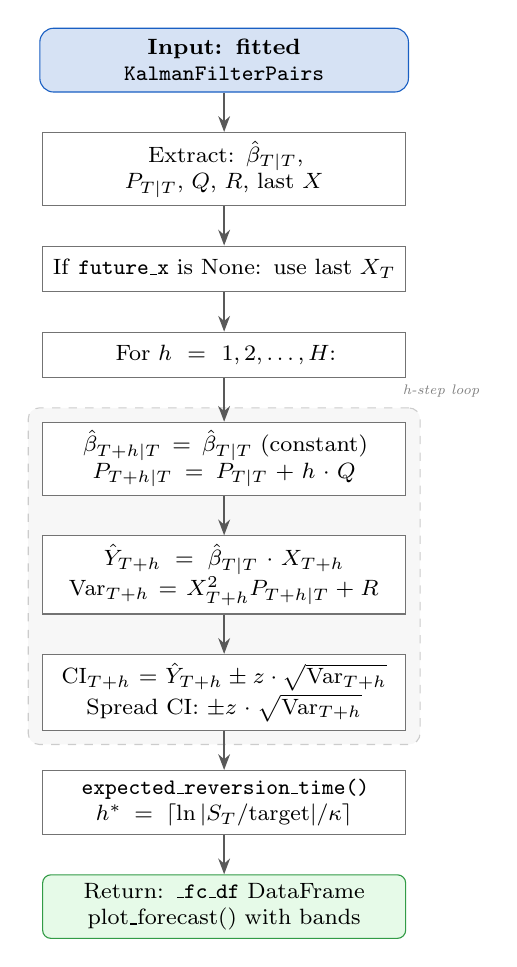
\begin{tikzpicture}[node distance=0.5cm,every node/.style={font=\scriptsize}]
  \node (in) [fc_start] {Input: fitted \texttt{KalmanFilterPairs}};
  \node (st) [fc_proc,below=of in]
    {Extract: $\hat\beta_{T|T}$, $P_{T|T}$, $Q$, $R$, last $X$};
  \node (st2)[fc_proc,below=of st] {If \texttt{future\_x} is None: use last $X_T$};
  \node (lp) [fc_proc,below=of st2]
    {For $h = 1, 2, \ldots, H$:};
  \node (bfc)[fc_proc,below=0.55cm of lp]
    {$\hat\beta_{T+h|T} = \hat\beta_{T|T}$ (constant)\\
     $P_{T+h|T} = P_{T|T} + h\cdot Q$};
  \node (yfc)[fc_proc,below=of bfc]
    {$\hat{Y}_{T+h} = \hat\beta_{T|T}\cdot X_{T+h}$\\
     $\mathrm{Var}_{T+h} = X_{T+h}^2 P_{T+h|T} + R$};
  \node (ci) [fc_proc,below=of yfc]
    {$\mathrm{CI}_{T+h} = \hat{Y}_{T+h} \pm z\cdot\sqrt{\mathrm{Var}_{T+h}}$\\
     Spread CI: $\pm z\cdot\sqrt{\mathrm{Var}_{T+h}}$};
  \node (rev)[fc_proc,below=of ci]
    {\texttt{expected\_reversion\_time()}\\ $h^* = \lceil\ln|S_T/\text{target}|/\kappa\rceil$};
  \node (out)[fc_out,below=0.5cm of rev]
    {Return: \texttt{\_fc\_df} DataFrame\\
     plot\_forecast() with bands};
  \draw[arr](in)--(st); \draw[arr](st)--(st2); \draw[arr](st2)--(lp);
  \draw[arr](lp)--(bfc); \draw[arr](bfc)--(yfc); \draw[arr](yfc)--(ci);
  \draw[arr](ci)--(rev); \draw[arr](rev)--(out);
  \begin{pgfonlayer}{background}
    \node[draw=gray!40,fill=gray!6,dashed,rounded corners=4pt,
          fit=(bfc)(yfc)(ci),inner sep=5pt,
          label={[font=\tiny\itshape,gray]above right:h-step loop}]{};
  \end{pgfonlayer}
\end{tikzpicture}
}
\caption{Execution flowchart for \texttt{KalmanForecaster.forecast()}.}
\end{figure}

%=============================================================================
\section{Python Implementation}
%=============================================================================

\begin{tcolorbox}[codebox={forecast\_beta and forecast\_P}]
\begin{lstlisting}[style=pythonplain]
def forecast_beta(self, steps: int) -> np.ndarray:
    # Formula 1: beta constant under random walk
    return np.full(steps, self._beta_T)

def forecast_P(self, steps: int) -> np.ndarray:
    # Formula 2: P grows linearly with h
    h_arr = np.arange(1, steps + 1)
    return self._P_T + h_arr * self._Q
\end{lstlisting}
\end{tcolorbox}

\begin{tcolorbox}[codebox={forecast() --- main method}]
\begin{lstlisting}[style=pythonplain]
def forecast(self, steps=20, future_x=None):
    if future_x is None:
        future_x = np.full(steps, self._last_x)
    x_ext = self._extend_x(future_x, steps)
    beta_fc = self.forecast_beta(steps)    # constant
    P_fc    = self.forecast_P(steps)       # growing
    y_fc    = beta_fc * x_ext             # Formula 3
    y_var   = x_ext**2 * P_fc + self._R  # Formula 4
    y_se    = np.sqrt(y_var)
    spread_upper =  self._z_crit * y_se  # Formula 6
    spread_lower = -self._z_crit * y_se
    # Build DataFrame and return
\end{lstlisting}
\end{tcolorbox}

\begin{tcolorbox}[codebox={expected\_reversion\_time()}]
\begin{lstlisting}[style=pythonplain]
def expected_reversion_time(self):
    innovations = np.array([s.innovation
                    for s in self._kf.states])
    if len(innovations) > 2:
        # Estimate kappa from innovation AR(1)
        acf1 = np.corrcoef(innovations[:-1],
                           innovations[1:])[0,1]
        if -1 < acf1 < 1 and acf1 < 0:
            kappa = -np.log(abs(acf1))
            h_star = ceil(
                log(|S_T|/target) / kappa)
            return max(1, min(h_star, steps))
\end{lstlisting}
\end{tcolorbox}

%=============================================================================
\section{Filter vs.\ Forecast: Key Distinction}
%=============================================================================

\begin{center}
{\small
\begin{tabular}{@{}lcc@{}}
\toprule
Property & Filter ($t \leq T$) & Forecast ($t > T$)\\\midrule
Data used & $Y_1,\ldots,Y_t$ & $Y_1,\ldots,Y_T$ (no new)\\
Step run & Predict + Update & Predict only\\
$\hat\beta$ changes & Yes (per update) & No (constant)\\
$P$ behaviour & Decreases on update & Increases by $Q$\\
Spread & $Y_t - \hat\beta_{t|t}X_t$ & Zero (expected)\\
Use case & Live trading & Position sizing, risk\\\bottomrule
\end{tabular}
}
\end{center}

%=============================================================================
\section{Practical Guide: Using Forecasts for Trading}
%=============================================================================

\begin{tcolorbox}[notebox={When to Act on Forecasts}]
\begin{enumerate}\setlength\itemsep{1pt}
  \item \textbf{Entry check}: If current spread $|S_T|$ is large and
    $h^* < \text{max hold period}$, the trade is viable.
  \item \textbf{Exit planning}: At $h = h^*$, the spread is expected
    to reach near-zero.  Plan to close the position by then.
  \item \textbf{Position sizing}: The CI width at $h^*$ determines
    risk.  Narrow CI → larger position; wide CI → smaller.
  \item \textbf{Stop-loss}: If the forecast CI at $h=1$ exceeds the
    stop-loss spread level, do not enter the trade.
\end{enumerate}
\end{tcolorbox}

%=============================================================================
\section{Pipeline Position}
%=============================================================================

\begin{center}{\small
\begin{tabular}{@{}clp{2.5cm}@{}}
\toprule Step & Module & Output\\\midrule
6 & \texttt{kalman\_filter.py} & $\hat\beta_{T|T}$, $P_{T|T}$\\
6.1 & \texttt{smoother.py} & $\hat\beta_{t|T}$ (offline)\\
6.2 & \texttt{dynamic\_beta.py} & Full pipeline\\
\textbf{7} & \textbf{\texttt{kalman\_forecast.py}} & CI bands, $h^*$\\
7b & \texttt{vecm\_forecast.py} & Price level + spread\\
8 & \texttt{signal/pair\_signal.py} & Entry/exit signals\\
9 & \texttt{backtest/engine.py} & Strategy backtest\\
\bottomrule
\end{tabular}
}\end{center}

%=============================================================================
\section{Interview Preparation}
%=============================================================================

\begin{tcolorbox}[exbox={Key Interview Questions}]
\begin{enumerate}\setlength\itemsep{2pt}
  \item \textbf{Why is the forecast spread zero in expectation?}\\
    Because $\hat\beta_{T+h|T} = \hat\beta_{T|T}$ (random walk): the forecasted
    $Y$ and the hedged $X$ exactly cancel.  The model believes the pair is in
    equilibrium going forward.
  \item \textbf{Why does uncertainty grow linearly?}\\
    Each step adds $Q$ to $P$: $P_{T+h|T} = P_{T|T} + hQ$.  $Q$ represents
    the per-step variance of the $\beta$ random walk.
  \item \textbf{How does the CI help with position sizing?}\\
    Wider CI → more uncertainty → smaller position.  Kelly-style sizing:
    $f \propto \hat{S}_T^2 / \mathrm{Var}_{T+h^*}$.
  \item \textbf{What if future X is unknown?}\\
    The code uses the last observed $X_T$ as a flat projection.  In practice,
    one can use VECM forecasts of $X_{T+h}$ (from \texttt{vecm\_forecast.py}).
  \item \textbf{How is $\kappa$ estimated from innovations?}\\
    AR(1) of innovations: $\varepsilon_t = \rho\varepsilon_{t-1} + \xi_t$.
    $\kappa \approx -\ln|\hat\rho_1|$.  This links filter residuals to OU speed.
\end{enumerate}
\end{tcolorbox}

\end{document}
